\begin{questions}
\question{
Heteronuclear Diatomic Molecule
}
\begin{solution}
Now we are going to consider a heteronuclear diatomic molecule with two atoms A and B, and wavefunction
\begin{equation}
  \ket{\Psi} = c_A \ket{A} + c_B \ket{B}.
  \label{2:psi}
\end{equation}
using eqs. \ref{sch:1}, and \ref{2:psi}, we can do the following
\begin{equation}
  \begin{aligned}[b]
    \bra{A}\hat{H}\left( c_A\ket{A} + c_B \ket{B} \right) &= \bra{A} E \left( c_A\ket{A} + c_B \ket{B} \right), \\
    c_A\cancelto{E_A}{\braket{A|\hat{H}|A}} + c_B\cancelto{\beta}{\braket{A|\hat{H}|B}} &= c_AE\cancelto{1}{\braket{A|A}} + c_BE\cancelto{0}{\braket{A|B}}, \\
    c_A(E_A - E) + c_B\beta &= 0.
  \end{aligned}
  \label{2:sys:1}
\end{equation}
the same with $\bra{B}$
\begin{equation}
  \begin{aligned}[b]
    \bra{B}\hat{H}\left( c_A\ket{A} + c_B \ket{B} \right) &= \bra{B} E \left( c_A\ket{A} + c_B \ket{B} \right), \\
    c_A\cancelto{\beta}{\braket{B|\hat{H}|A}} + c_B\cancelto{E_B}{\braket{B|\hat{H}|B}} &= c_AE\cancelto{0}{\braket{B|A}} + c_BE\cancelto{1}{\braket{B|B}}, \\
    c_A\beta + c_B(E_B-E) &= 0.
  \end{aligned}
  \label{2:sys:2}
\end{equation}
So now the system to solve is
\begin{equation}
  \begin{bmatrix}
    E_A - E & \beta \\
    \beta & E_B - E
  \end{bmatrix}
  \begin{bmatrix}
    c_A \\
    c_B
  \end{bmatrix}
  =
  \begin{bmatrix}
    0 \\
    0
  \end{bmatrix}.
  \label{2:sys:full}
\end{equation}
The system has solution if
\begin{equation}
  \begin{vmatrix}
    E_A - E & \beta \\
    \beta & E_B - E
  \end{vmatrix} = 0,
  \label{2:det}
\end{equation}
and this means
\begin{equation}
  \begin{aligned}[b]
    0&=(E_A - E)(E_B - E) - \beta^2,\\
     &=E_AE_B - EE_B - EE_A + E^2 - \beta^2,\\
     &=E^2 + E(-1)(E_A + E_B) + (E_AE_B - \beta^2).
    \label{quad}
  \end{aligned}
\end{equation}
The solution to eq. \ref{quad} is
\begin{equation}
  \begin{aligned}[b]
    E_\pm &= \frac{E_B + E_A \pm \sqrt{(E_A + E_B)^2 - 4(E_AE_B - \beta^2)}}{2},\\
    &= \frac{E_B + E_A \pm \sqrt{E_A^2 + E_B^2 + 2E_AE_B - 4E_AE_B + 4\beta^2)}}{2},\\
    &= \frac{E_B + E_A \pm \sqrt{(E_A - E_B)^2 + 4\beta^2)}}{2},\\
    &= \frac{E_B + E_A}{2}\pm \sqrt{\left(\frac{E_A - E_B}{2}\right)^2 + \beta^2},\\
    &= \hlgreen{\frac{E_B + E_A}{2}\pm \sqrt{\Delta^2 + \beta^2},}
  \end{aligned}
\end{equation}
where in the last term we used
\begin{equation}
  \Delta = \frac{E_A - E_B}{2}.
\end{equation}

Now that we know this, obtaining the coefficients is really easy. Let's take for example eq. \ref{2:sys:1} and isolate $c_B$
\begin{equation}
  \begin{aligned}[b]
    c_A(E_A - E) + c_B\beta = 0,\\
    \Rightarrow \hlgreen{c_B = -\frac{c_A (E_A - E)}{\beta}.}
  \end{aligned}
\end{equation}
Now we must remember that the normalization on this case when $\braket{A|B} = 0$ imposes $c_A^2 + c_B^2 = 1$, hence
\begin{equation}
  \begin{aligned}[b]
    1 &= c_A^2 + c_B^2 ,\\
    &=c_A^2 + c_A^2\left( \frac{E_A - E}{\beta}\right)^2,\\
    &= c_A^2 \left(1+\left( \frac{E_A - E}{\beta}\right)^2\right).\\
    \Rightarrow \hlgreen{c_A} &\hlgreen{= \frac{1}{\sqrt{1+\left( \frac{E_A - E}{\beta}\right)^2}}.}
  \end{aligned}
\end{equation}
Now we just need to plug the energy of the bonding state ($E_-$) or the anti-bonding state ($E_+$), in order to get the coefficients we are looking for.

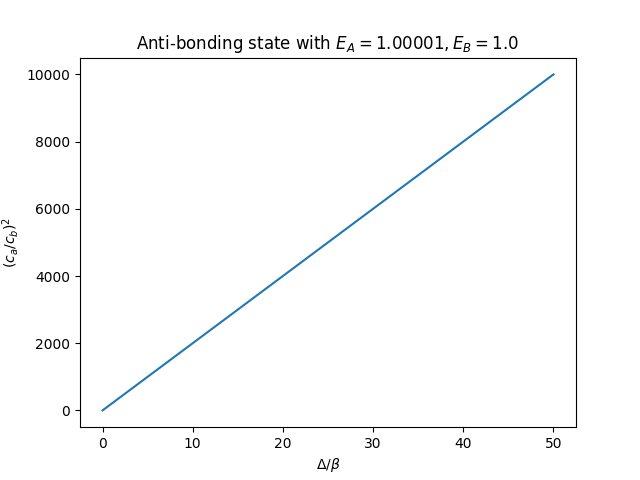
\includegraphics[width=75mm]{anti-1-mal.png}
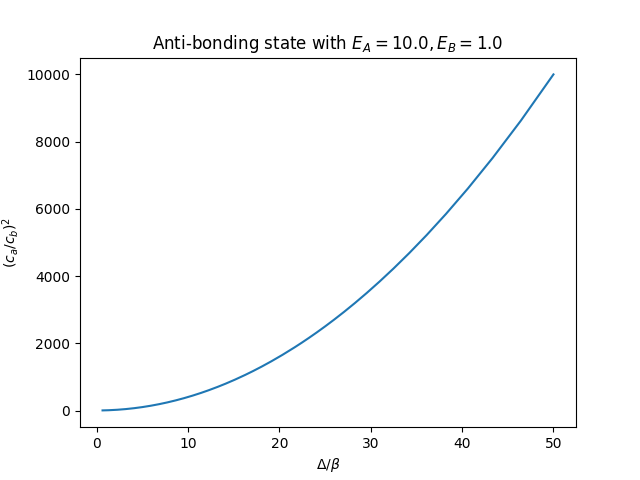
\includegraphics[width=75mm]{anti-10-mal.png}

\hspace{3.6cm}a)\hspace{7.5cm}b)

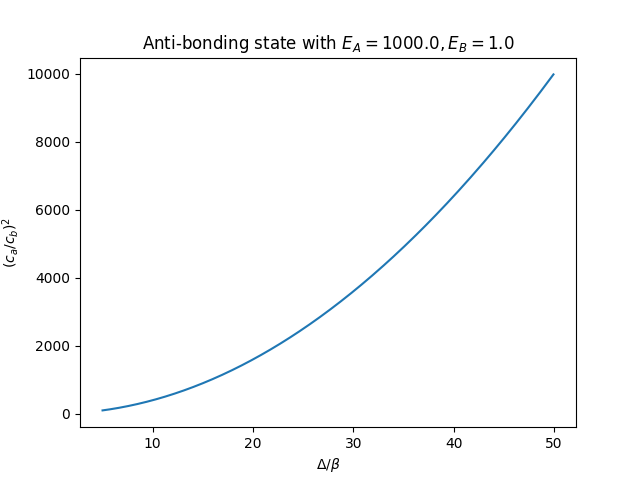
\includegraphics[width=75mm]{anti-1000-mal.png}
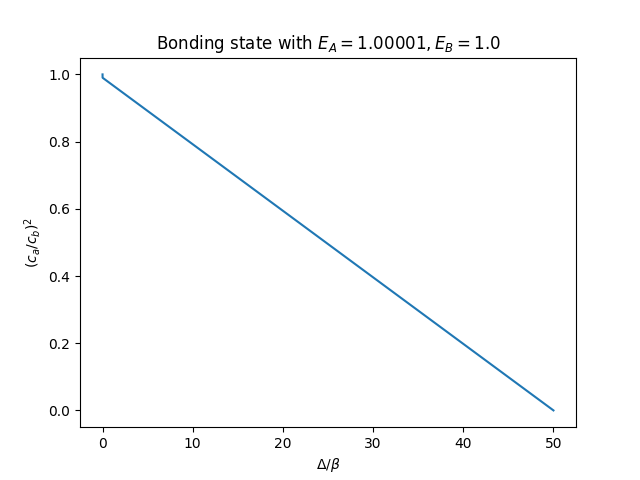
\includegraphics[width=75mm]{bond-1-mal.png}

\hspace{3.6cm}c)\hspace{7.5cm}d)

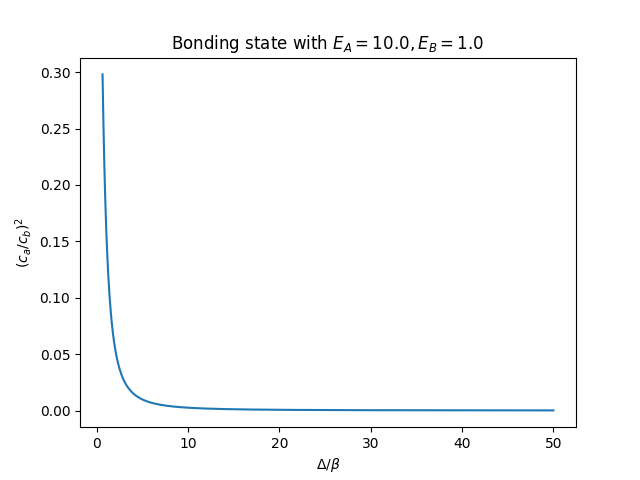
\includegraphics[width=75mm]{bond-10-mal.png}
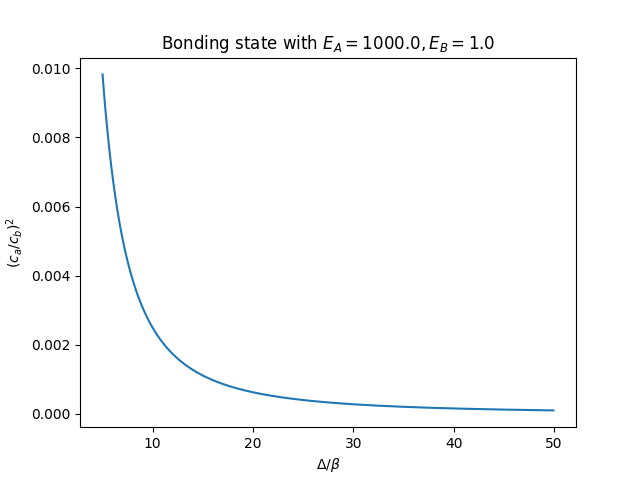
\includegraphics[width=75mm]{bond-1000-mal.png}\label{bondplots}

\hspace{3.6cm}e)\hspace{7.5cm}f)

 \captionof{figure}{$(c_a/c_b)^2$ plotted for the anti-bonding (a,b,c) and the bonding states (d,e,f)}

 As we can see in Fig. \ref{bondplots} ... \textit{to be continued}
\end{solution}
\end{questions}
